%        File: vt_hyperparam_viz.tex
%     Created: Fri Jun 22 09:00 AM 2018 C
% Last Change: Fri Jun 22 09:00 AM 2018 C
%
\documentclass[a4paper]{article}
\usepackage{graphicx}
\title{Visualization for Hyperparameter Optimization}
\author{Nathan Wycoff}

\begin{document}
\maketitle

\section{Introduction}

Hyperparameter optimization is an unsolved problem in theoretical machine learning and an important practical consideration. Many efforts exist to conduct this optimization automatically, see, e.g., https://cloud.google.com/automl/, or https://bayesopt.github.io/. Another approach would be to enhance a human's ability to manually conduct this optimzation. In this document, we'll outline a general method to do this via visual examination of assumptions.

\section{Framework}

The proposed framework is best presented as consisting of several components. Under the framework, each of these needs to be specified by the end user. In general, this would involve the end user writing code. However, the hope is that components are generalizable enough that the user can simply choose between existing components.

\subsection{Technologies}

This project is written in the R programming language, and uses the Shiny package to dynamically generate front end to user specifications. It is implemented as an R package, allowing easy, OS independent installation, and exposes a single function, ``remote\_run", which allows the user to create a custom debugging environment for their machine learning tool.

\subsection{A Machine Learning Algorithm for Training}

The user needs to specify how the algorithm will interact with the data to fit the model, this process being mediated by the hyperparameters. The backend will run the specified algorithm once for each user specified hyperparameter combination. This function is the argument ``get\_model\_fit".

\subsection{A Latent Representation}

In order to examine the machine learning model's assumptions, suitable quantities need to be determined. This is, in general, the hardest part of the visualization process: determining what to visualize. The idea is to visualize the input data through the eyes of the model. By default, for supervised models, this means invoking R's ``predict" function, which allows us to visualize what the model has predicted for each input data, but other options are possible. This step is critical to the success of the visualization.

\subsection{A Dimensionality Reduction Scheme}

Once we've determined a latent representation, we need to turn it into a scatterplot. This may be accomplished via dimensionality reduction. By default, the algorithm performs PCA, a very quick and general method, but others are possible, such as MultiDimensional Scaling (MDS).

\subsection{Hyperparameter Specification}

The entire point of the project is to optimize a set of hyperparameters. The user may specify 1 or more hyperparameters, telling us whether it is continuous valued, integer value, or categorical, and may specify lower or upper bounds on the params. A frontend will be automatically created to reflect this information.

\section{Examples}

In this section, we'll go through two examples, executed on an early version of the software.

\subsection{Normal Mixture Model}

Normal Mixture models are clustering algorithms. The only hyperparameter is the number of clusters to look for, which must be user specified. In this example, the latent space representation is a residual of sorts: each data point has subtracted from it the mean of its cluster. If we still see clustering behaviour, it means that we don't have enough clusters.

We'll being by trying two clusters. Coloration is due to the assigned cluster:

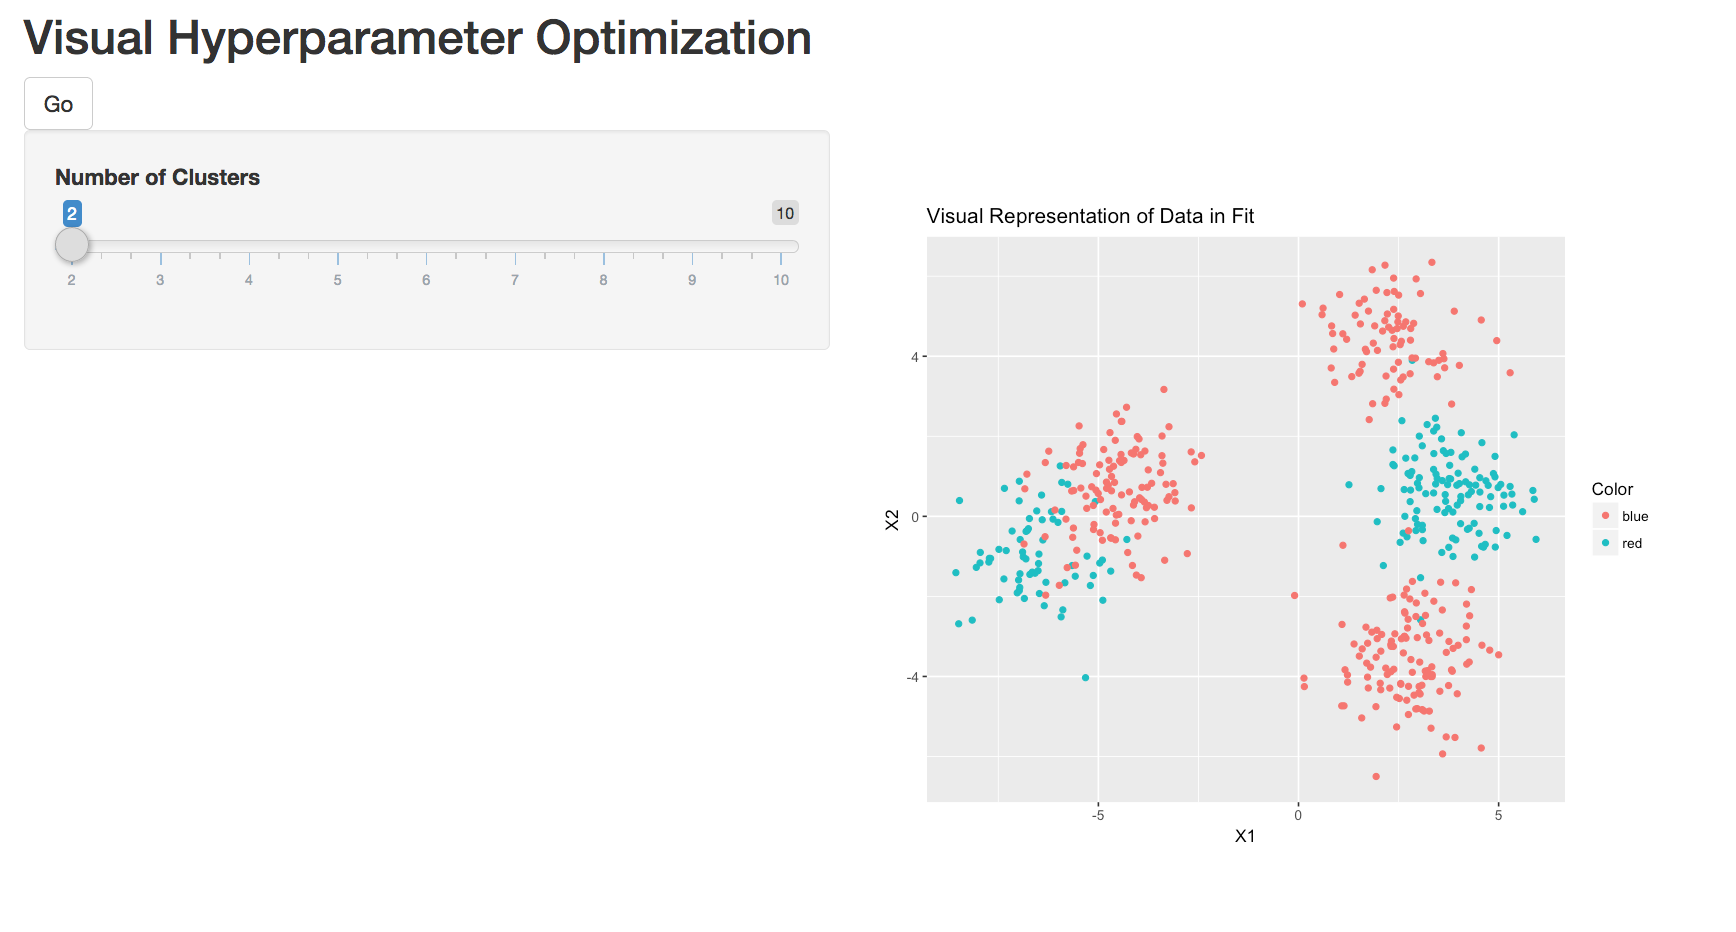
\includegraphics[width=\linewidth]{../images/norm_mix_1.png}

We notice that our latent representation still has structure in it, so we increment th cluster count to 5:

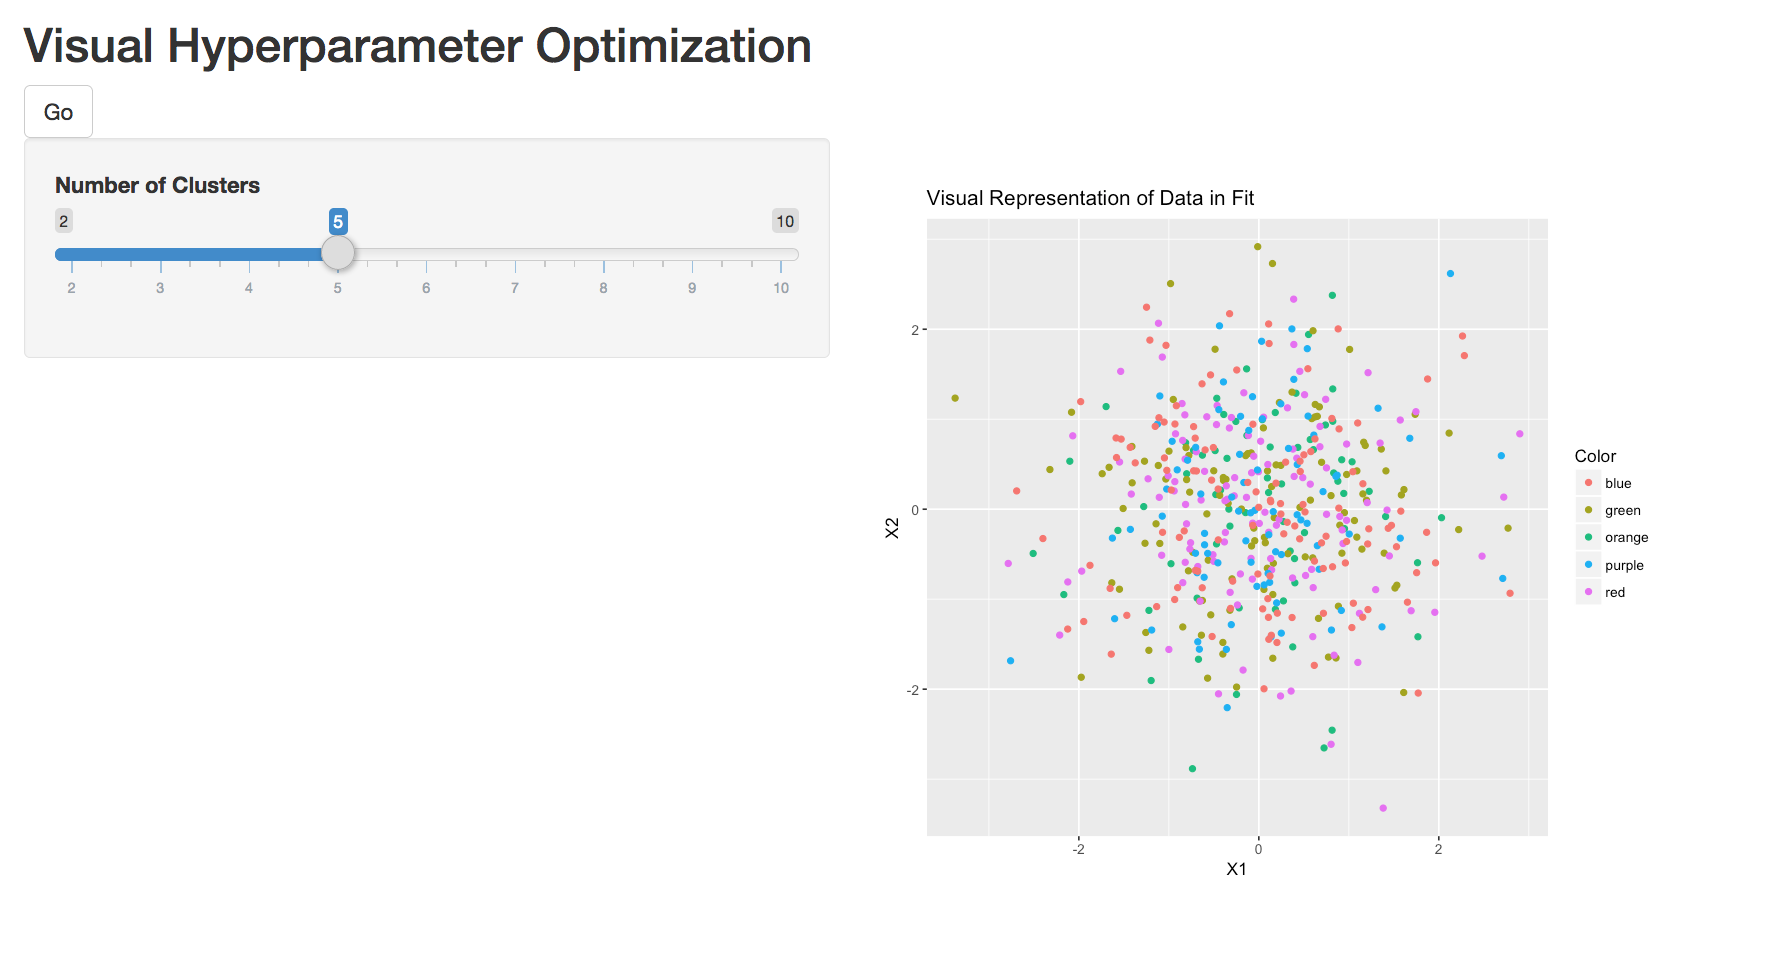
\includegraphics[width=\linewidth]{../images/norm_mix_2.png}

There is no longer any structure in the data, so we know we have enough clusters. We could go down to 4 to confirm that there is still structure then. These data are simulated, and have 5 clusters in truth.

In this example, we've chosen a latent representation that helps us determine our hyperparameters.

\subsection{Convnet}

Convolutional Neural Networks are image classification algorithms. The network structure must be decided upon, which involves very many hyperparameters. There are also various regularization parameters, such as dropout rate or l1/l2 penalties, as well as optimizer characteristics, such as momentum, sgd batch size, etc. But for this example, we will focus on rectangular fully connected layers, and let the convolutional layers be. We'll allow the user to pick how many nodes are in each fully connected layer, as well as how many fully connected layers there are. 

The latent space will be the activation functions of the last hidden layer, and the dimensionality reduction technique will be PCA.

The dataset is a reduced version of the MNIST data, with only the numbers 0, 1, 4, and 7:

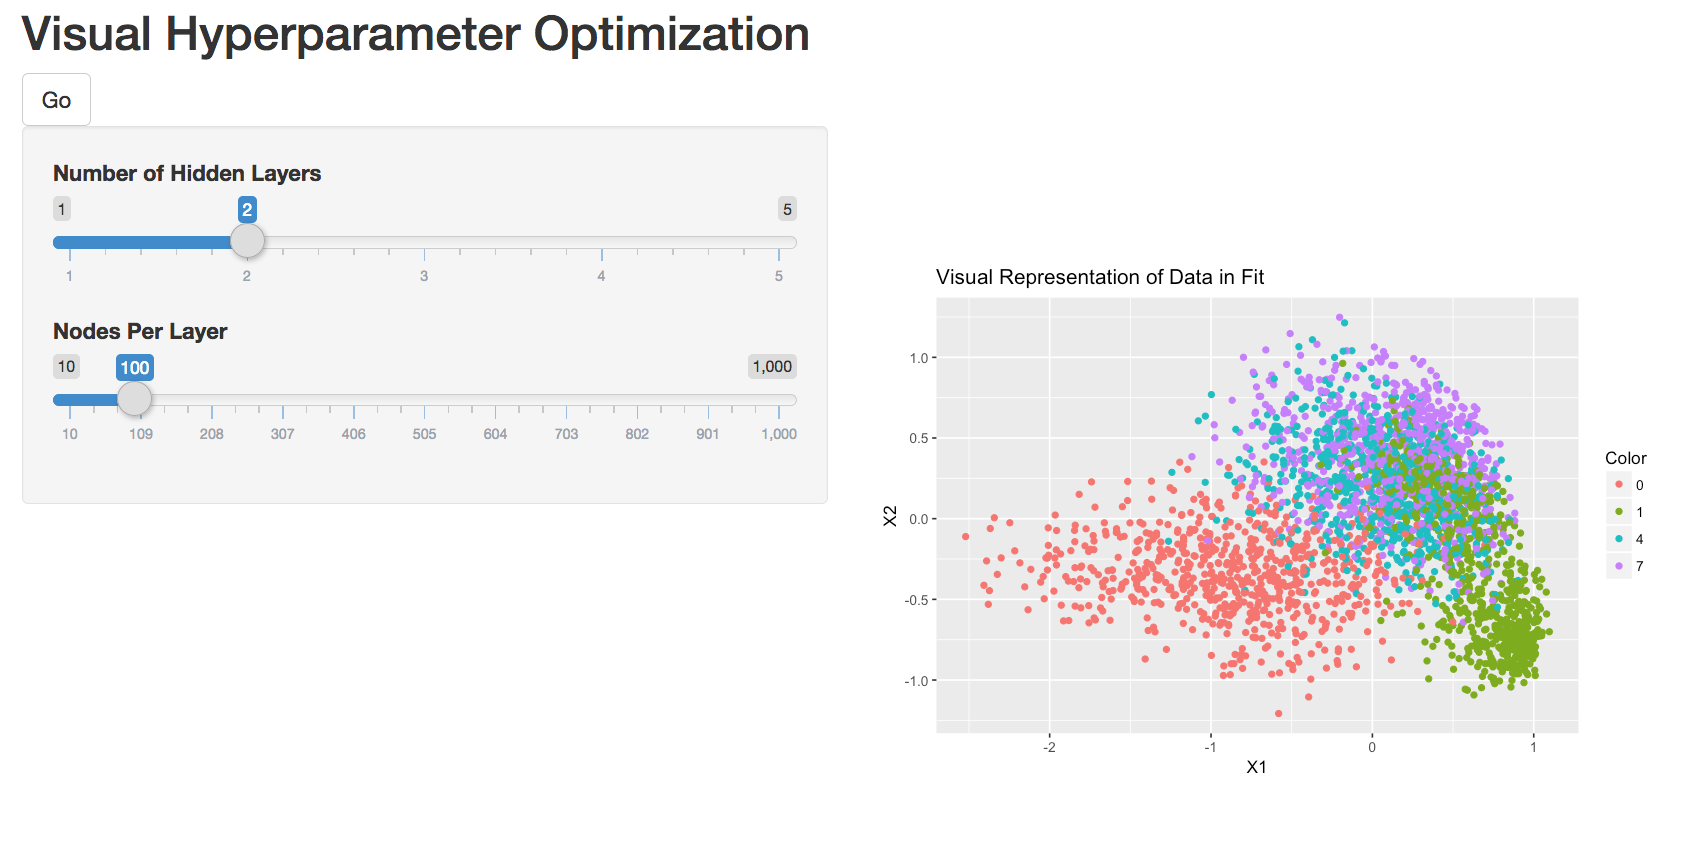
\includegraphics[width=\linewidth]{../images/nnet.png}

Part of the MNIST data's popularity is due to how intuitive it is. However, this certainly isn't the case for all data to which CNN's are applied. In this example, we can see how the visualization can help us understand the data. We see that the representation of 0 characters is spread out fairly wide, while the representations for 1s are, for the most part, concentrated in the lower right (though some are scattered around). So we learn that there is, according to the CNN, much variance in observed 0's, and less variance in 11's, though there are outliers. 4 and 7, on the other hand, are projected right on top of one another. This tells us that they look alike. In the context of these data, that 4 and 7 look alike is already known, but in general, there may be little \textit{a priori} understanding of the data. This tool can help us build that understanding.

It is important to recognize that confusion between two classes in the plot is not the same as confusion by the classifier. In this case, though 4 and 7 are projected directly on top of one another, the classifier still has 99\%+ accuracy rate. This is because though the data are linearly separable in the origin high dimensional latent space, they are not linearly separable in 2D.



\end{document}
